\documentclass[10pt]{beamer}
\usetheme[progressbar=frametitle]{metropolis}
\usepackage{appendixnumberbeamer}
\usepackage{booktabs}
\usepackage[scale=2]{ccicons}
% \usepackage[ngerman]{babel}
\usepackage{graphicx} 
% \graphicspath{ {images/}  {../images/} }
\usepackage{tikz} 
\usepackage{wrapfig}
%\usepackage[utf8]{inputenc}
%\usepackage[T1]{fontenc}
\usepackage{moreverb}
\usepackage[backend=biber]{biblatex}   
\addbibresource{content/cites.bib}
%\bibliography{content/cites.bib}
\usepackage{textcomp}
%\usepackage{fontspec}
%\setsansfont{Fira Sans}
\usepackage{hyperref}
\renewcommand*{\bibfont}{\scriptsize}
%\usepackage{caption}
%\captionsetup[figure]{labelformat=empty}% redefines the caption setup of the figures environment in the beamer class.

\title{Mid-term Presentation}
\author{Samy Dafir, András Czuczi, Andreas Lindlbauer} %#nohomo
\date{}
\begin{document}

\begin{frame}
	\maketitle 
\end{frame}

%%%%%%%%%%%%%%%%%%%%%%%%%%%%%%%%%%%%%%%%%%%%%%%%%%%%%%%%%%%%%%%%%%%%%%%%%%%%%%%%%%%%%%%%%%%%%%%%

\begin{frame}{Overview}
	\tableofcontents
\end{frame}

%%%%%%%%%%%%%%%%%%%%%%%%%%%%%%%%%%%%%%%%%%%%%%%%%%%%%%%%%%%%%%%%%%%%%%%%%%%%%%%%%%%%%%%%%%%%%%%%

\section{Summary of subnetTALK}

%%%%%%%%%%%%%%%%%%%%%%%%%%%%%%%%%%%%%%%%%%%%%%%%%%%%%%%%%%%%%%%%%%%%%%%%%%%%%%%%%%%%%%%%%%%%%%%%

\begin{frame}{Human Building Interaction by Selena Savić I.} %%maybe not displayed
	\begin{itemize}
        \pause{}
		\item Human Building Interaction (HBI) focuses on resources and therefore on budgeting
		\pause{}
		\item Goal is to end the talk about whether resources are (in)finite
		\pause{}
		\item Scarcity of resources (whether artificial or not) has an impact on the design
		\pause{}
		\item Just because something is not scarce, no overusage is recommended (eg. WiFi and routers)
	\end{itemize}	
\end{frame}

%%%%%%%%%%%%%%%%%%%%%%%%%%%%%%%%%%%%%%%%%%%%%%%%%%%%%%%%%%%%%%%%%%%%%%%%%%%%%%%%%%%%%%%%%%%%%%%%

\begin{frame}{Human Building Interaction by Selena Savić II.} %% ``ć`` maybe not displayed
	\begin{itemize}
        \pause{}
		\item Computation has an impact on design of buildings -> smart buildings
		\pause{}
		\item Intelligent walls: optimize bandwith usage
		\pause{}
		\item RAM house: a prototype partially made of Radar Absolvent Material -> airplane mode for your house
		\pause{}
		\item Smart home: home expects user to do something (eg. use less energy at given time)
		\pause{}
		\item 
	\end{itemize}	
\end{frame}

%%%%%%%%%%%%%%%%%%%%%%%%%%%%%%%%%%%%%%%%%%%%%%%%%%%%%%%%%%%%%%%%%%%%%%%%%%%%%%%%%%%%%%%%%%%%%%%%
\section{Main findings from literature review}

%%%%%%%%%%%%%%%%%%%%%%%%%%%%%%%%%%%%%%%%%%%%%%%%%%%%%%%%%%%%%%%%%%%%%%%%%%%%%%%%%%%%%%%%%%%%%%%%

\begin{frame}{Intersection of architecture and interaction design}
	\metroset{block=fill}
	\begin{block}{Focus of space and architecture in interfaces}
	\begin{itemize}
        \pause{}
		\item Interaction with space instead of stuff
        \pause{}
		\item Media fa\c{c}ades
        \pause{}
		\item Architectural and spatial metaphors in interfaces
    \end{itemize}	
	\end{block}

    \pause{}
	\metroset{block=fill}
	\begin{block}{Connections between interaction design, technology and architecture}
	\begin{itemize}
        \pause{}
		\item Technology for architecture
        \pause{}
		\item Technology embedded in architecture
        \pause{}
		\item Architectonic technology
        \pause{}
        \item Architectonic interaction design
	\end{itemize}	
	\end{block}
\end{frame}


\begin{frame}{Adaptable architecture and feedback loops}
	\metroset{block=fill}
	\begin{block}{Make buildings more interactive and adaptable to human needs}
	\begin{itemize}
        \pause{}
		\item More interactive capabilities have impact
        \pause{}
		\item ``Responsive Places'' change according to occupants needs
        \pause{}
        \item Enhance connectivity to smart devices
        \pause{}
        \item Buildings and their use change over time, allow better appropriation and renovation
	\end{itemize}	
	\end{block}

    \pause{}
	\metroset{block=fill}
	\begin{block}{Feedback loop between human behavior and architecture}
	\begin{itemize}
        \pause{}
		\item Focus on feedback loop between humans and buildings
        \pause{}
		\item Relate movement of people to movement in architecture
	\end{itemize}	
	\end{block}

\end{frame}

%%%%%%%%%%%%%%%%%%%%%%%%%%%%%%%%%%%%%%%%%%%%%%%%%%%%%%%%%%%%%%%%%%%%%%%%%%%%%%%%%%%%%%%%%%%%%%%%

\section{Most interesting findings from SOTA}

%%%%%%%%%%%%%%%%%%%%%%%%%%%%%%%%%%%%%%%%%%%%%%%%%%%%%%%%%%%%%%%%%%%%%%%%%%%%%%%%%%%%%%%%%%%%%%%%

\begin{frame}{SOTA Findings}
	\metroset{block=fill}
	\begin{block}{Main Developments}
	\begin{itemize}
		\item Simplification and Optimisation
		\item Comfort
		\item Privacy
		\item Health
		\item Dynamic Living Spaces
		\item Implicit Interactions
	\end{itemize}	
	\end{block}
\end{frame}


\begin{frame}{SOTA Findings}
	\metroset{block=fill}
	\begin{block}{Main idea behind the smart home}
		\begin{itemize}
		\item Make everyday life easier, more efficient, comfortable.
		\item Use technology to make our lives healthier.
		\item Adapt to shrinking living space
		\item Use technology for everything, but keep privacy
		\end{itemize}
	\end{block}

	\begin{exampleblock}{Additional Developments}
	\begin{itemize}
		\item Implicit interactions: Interacting without actually interacting
	\end{itemize}
\end{exampleblock}
	
\end{frame}


\section{Examples / Projects}


\begin{frame}{RAM House}
	\textbf{Dynamic Privacy}\\
	\vspace{3mm}
	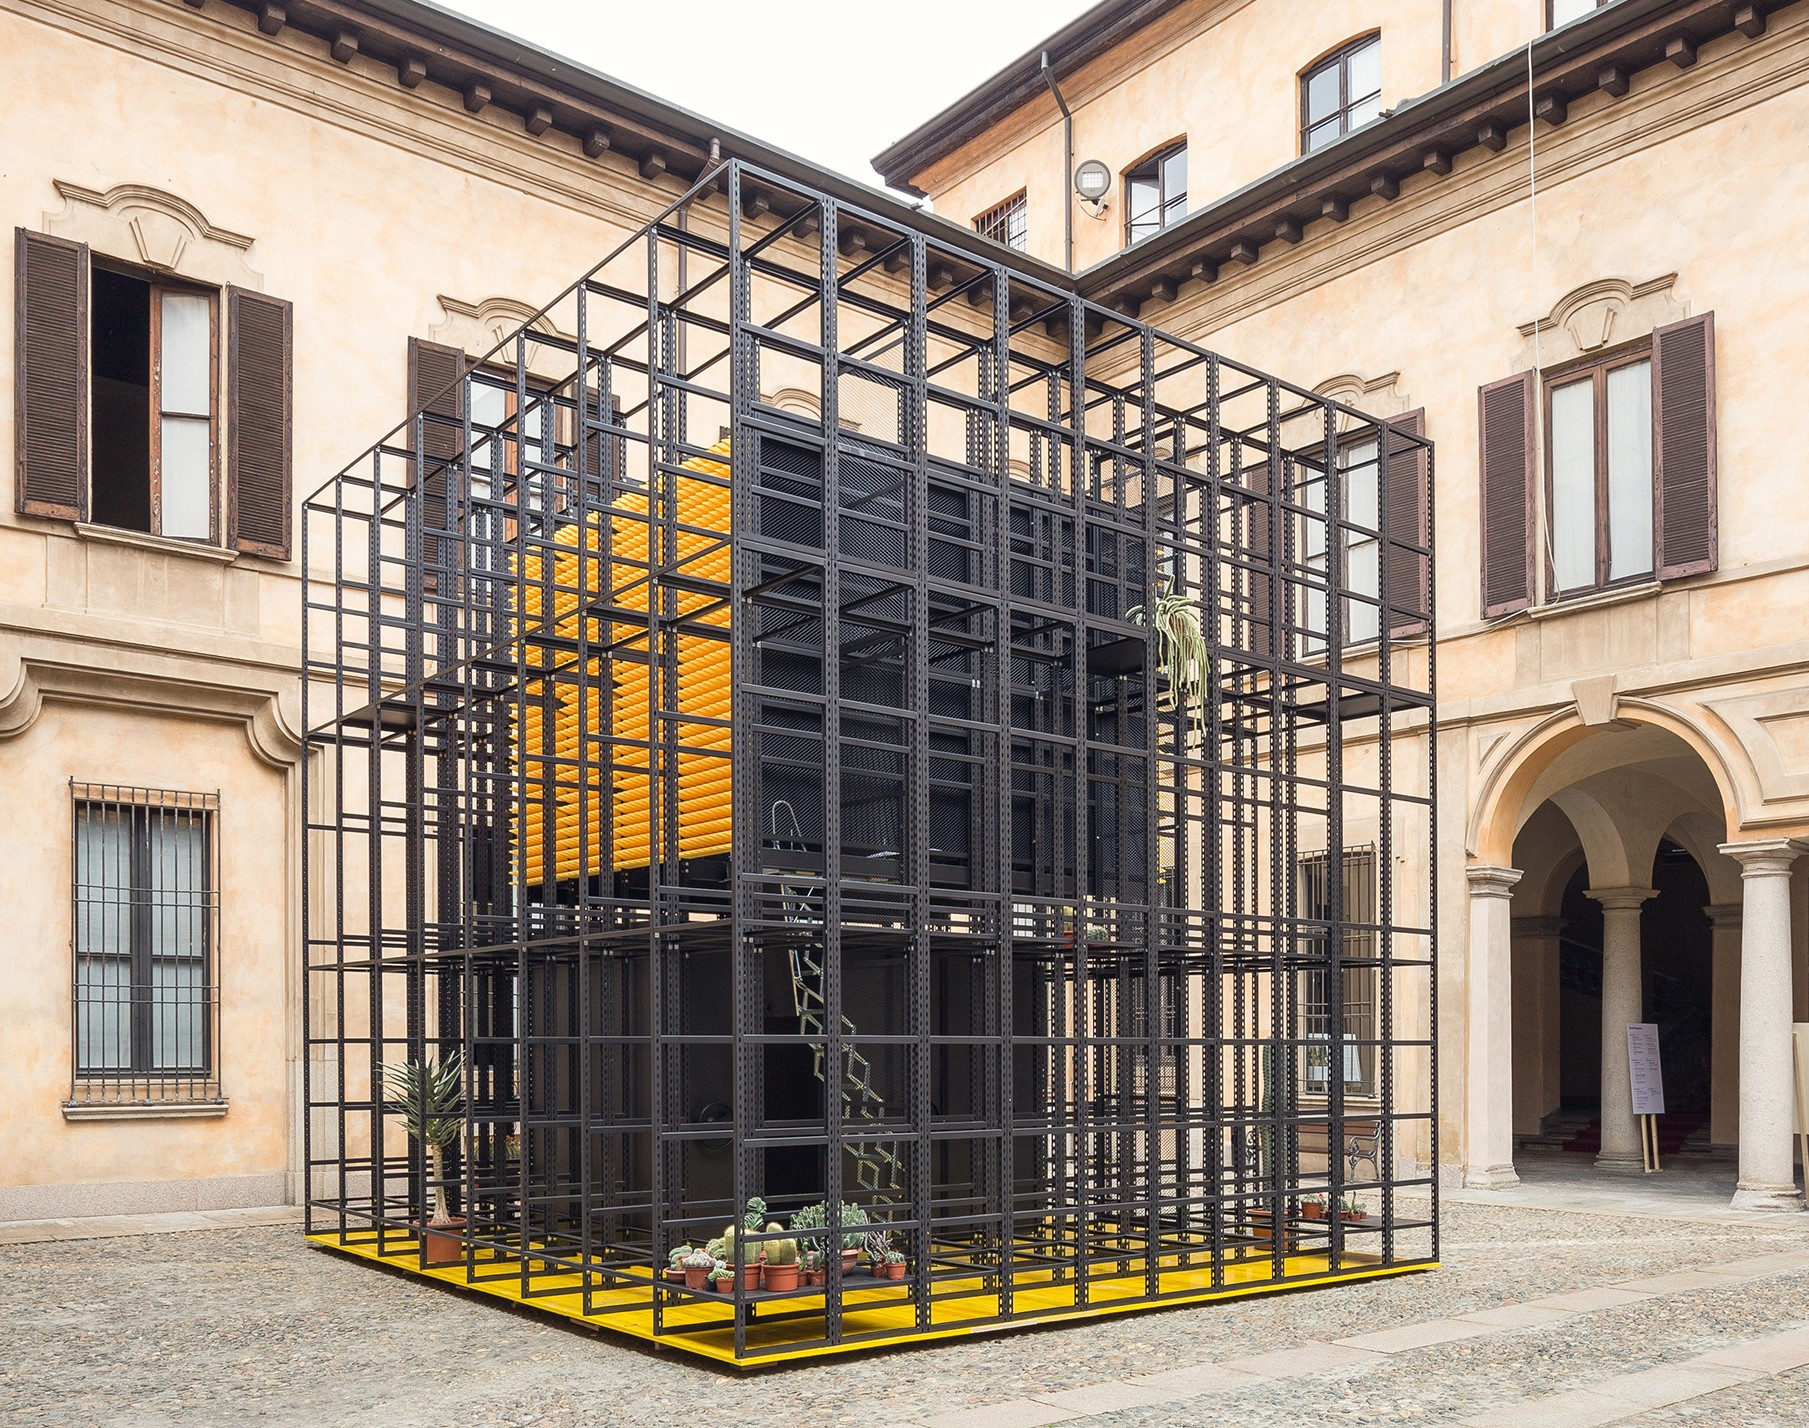
\includegraphics[width=0.7\textwidth]{images/1.jpg}
\end{frame}

\begin{frame}{Numi Toilet}
	\textbf{Comfort and Implicit Interaction}\\
	\vspace{3mm}
	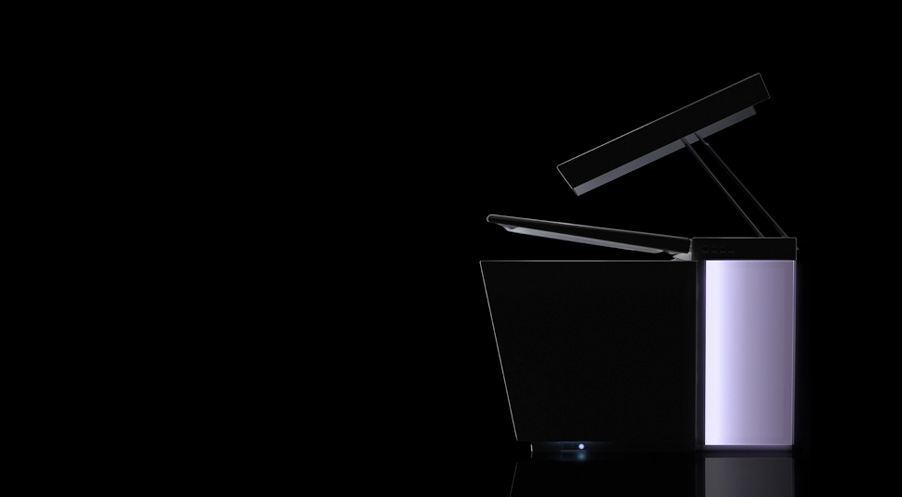
\includegraphics[width=\textwidth]{images/3.jpg}
\end{frame}

\begin{frame}{Numi Toilet}
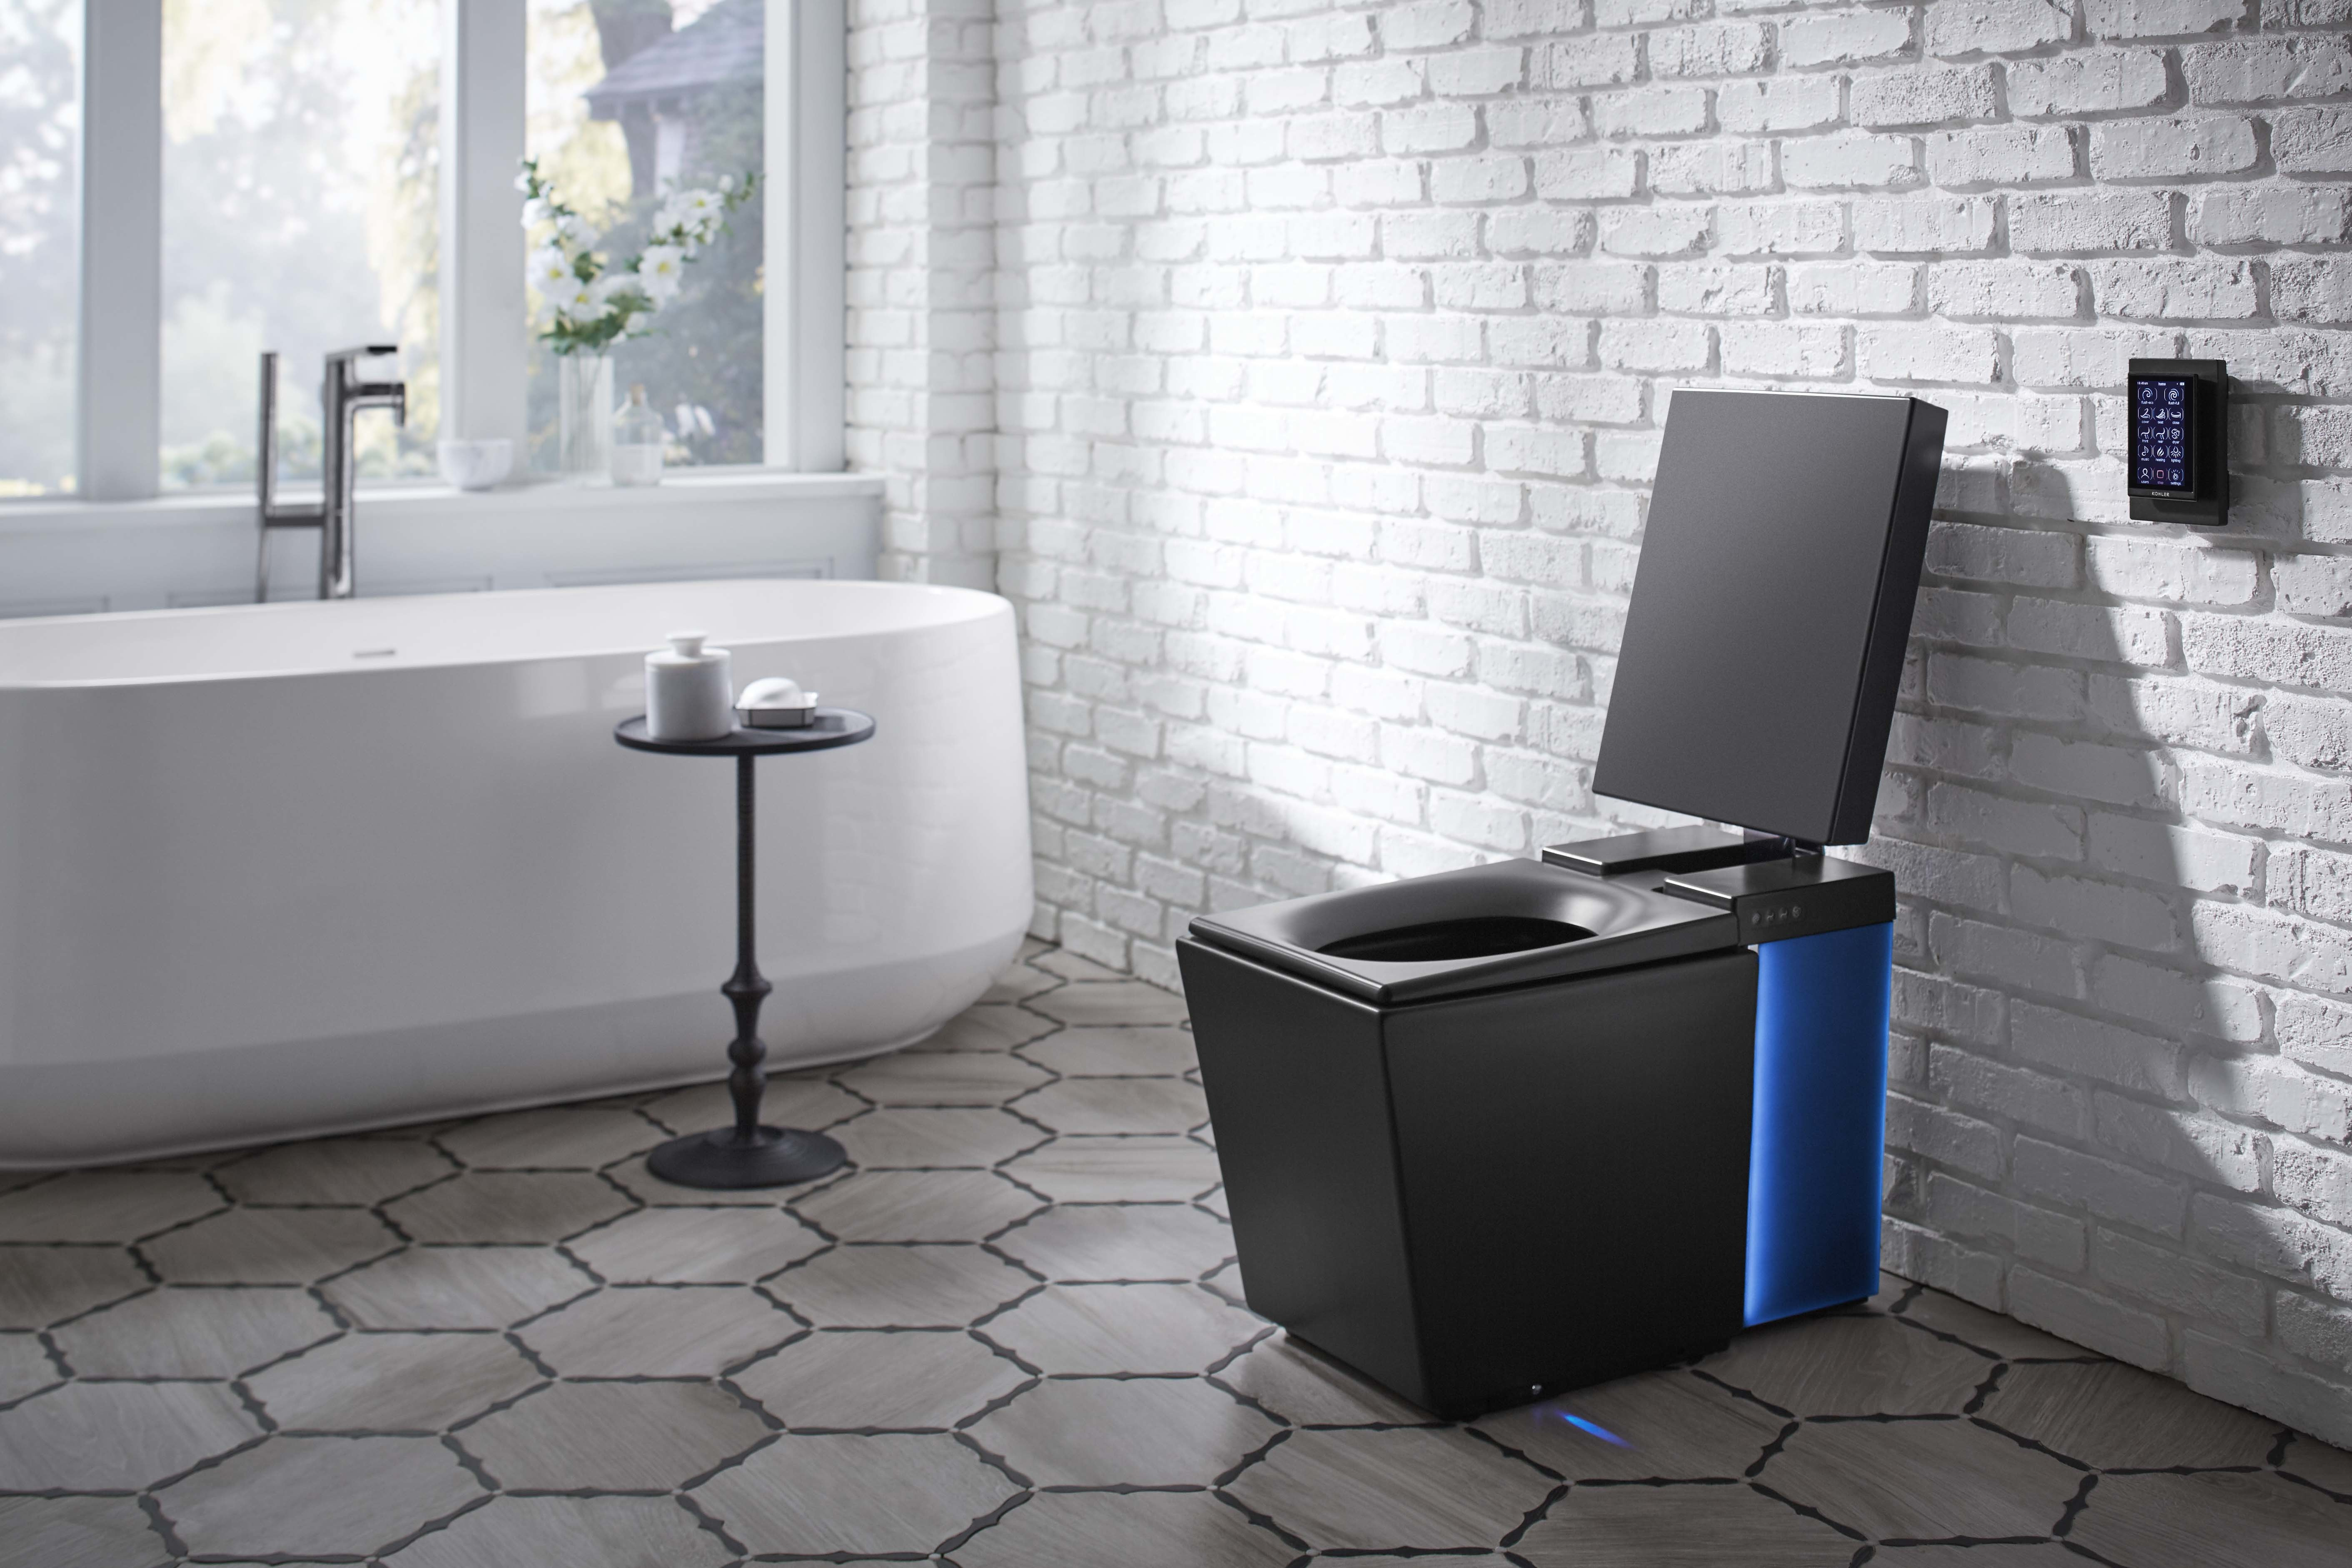
\includegraphics[width=\textwidth]{images/6.jpg}
\end{frame}

\begin{frame}{MIT CitiHome Project}
	\textbf{Dynamic Living Space}\\
	\vspace{3mm}
	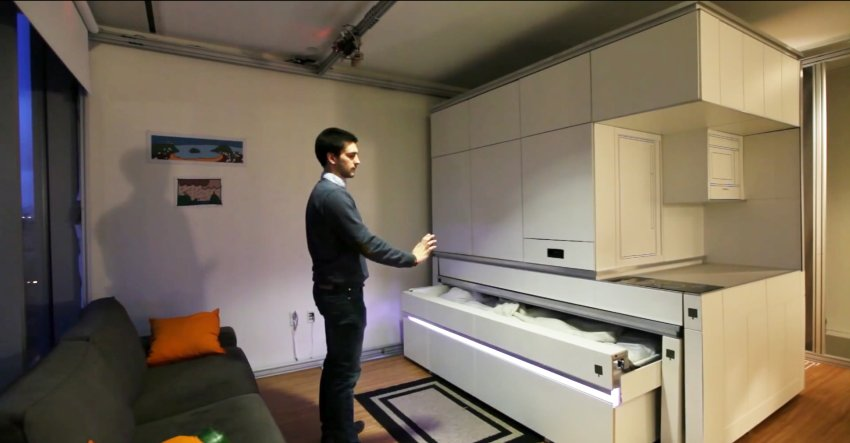
\includegraphics[width=\textwidth]{images/4.jpg}
\end{frame}

\begin{frame}{MIT CitiHome Project}
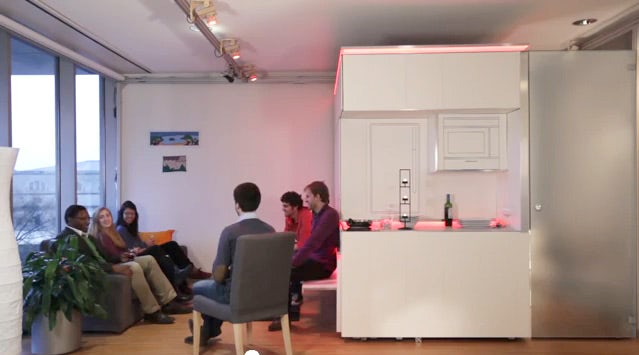
\includegraphics[width=\textwidth]{images/5.jpg}
\end{frame}

\begin{frame}{Infrascan Smart Toilet}
	\textbf{Health and Implicit Interaction}\\
	\vspace{3mm}
	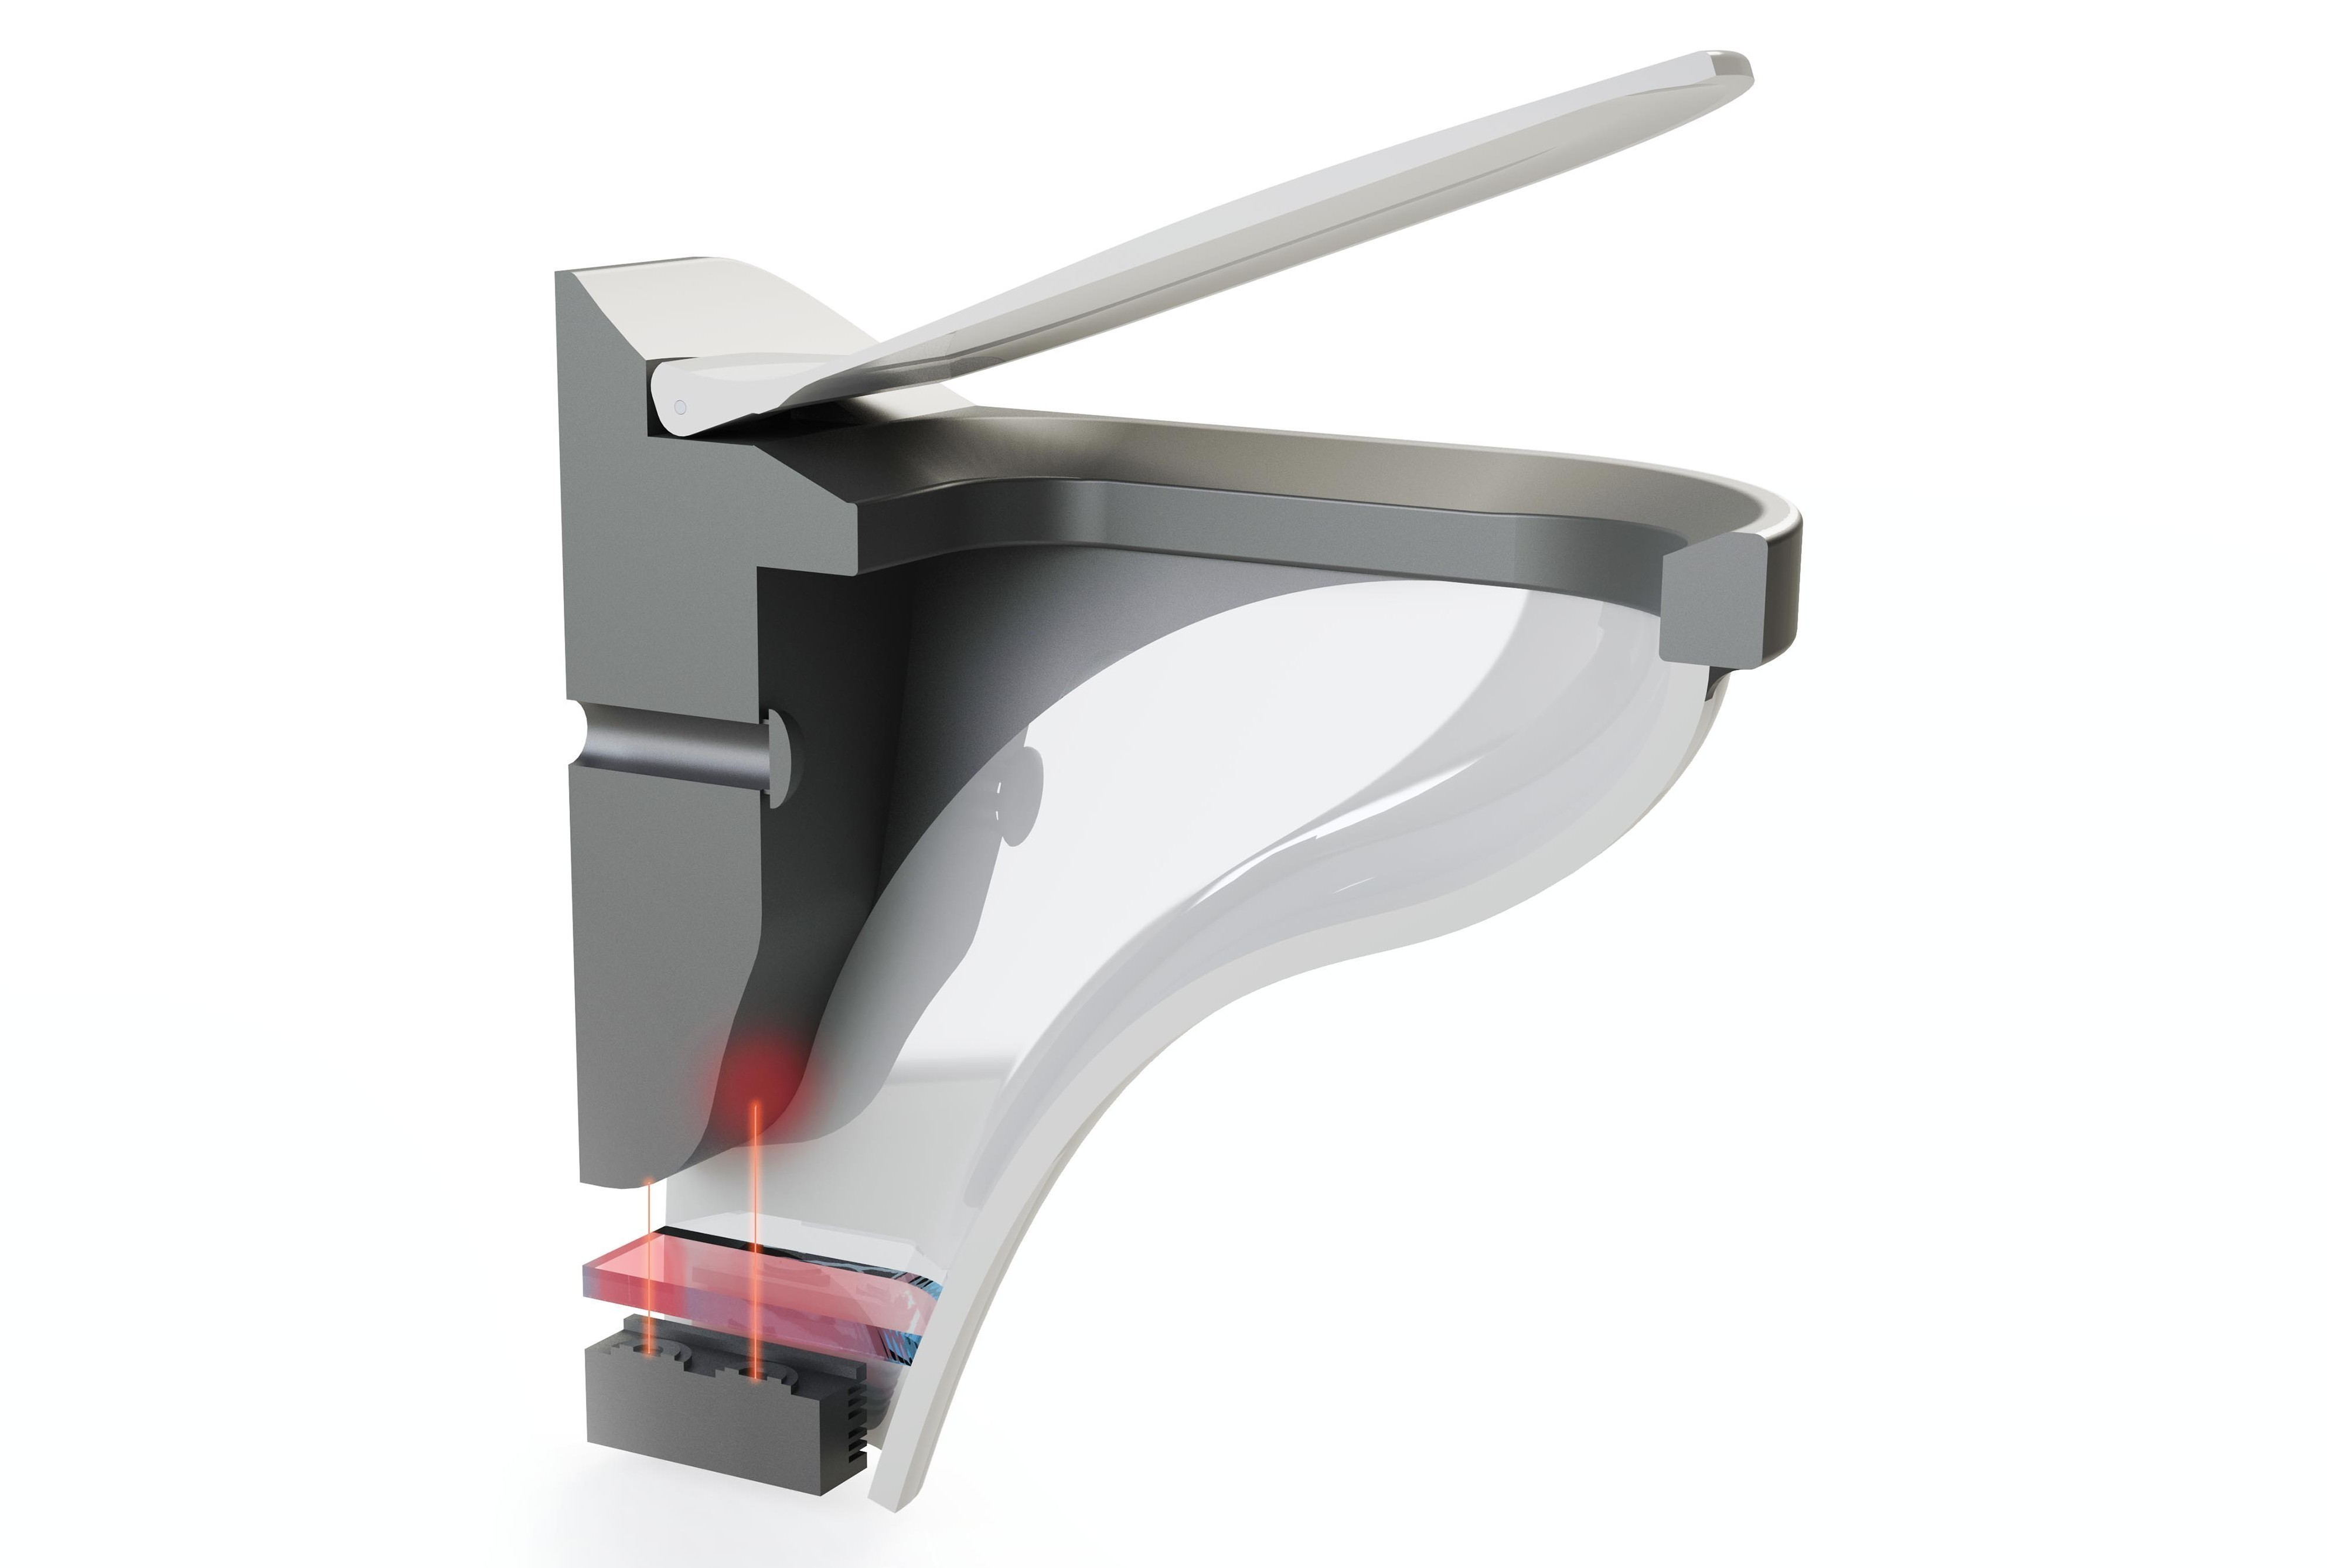
\includegraphics[width=\textwidth]{images/2.jpg}
\end{frame}

\begin{frame}{Intellithings RoomMe}
	\textbf{Simplification, Comfort, Implicit Interaction}\\
	\vspace{3mm}
	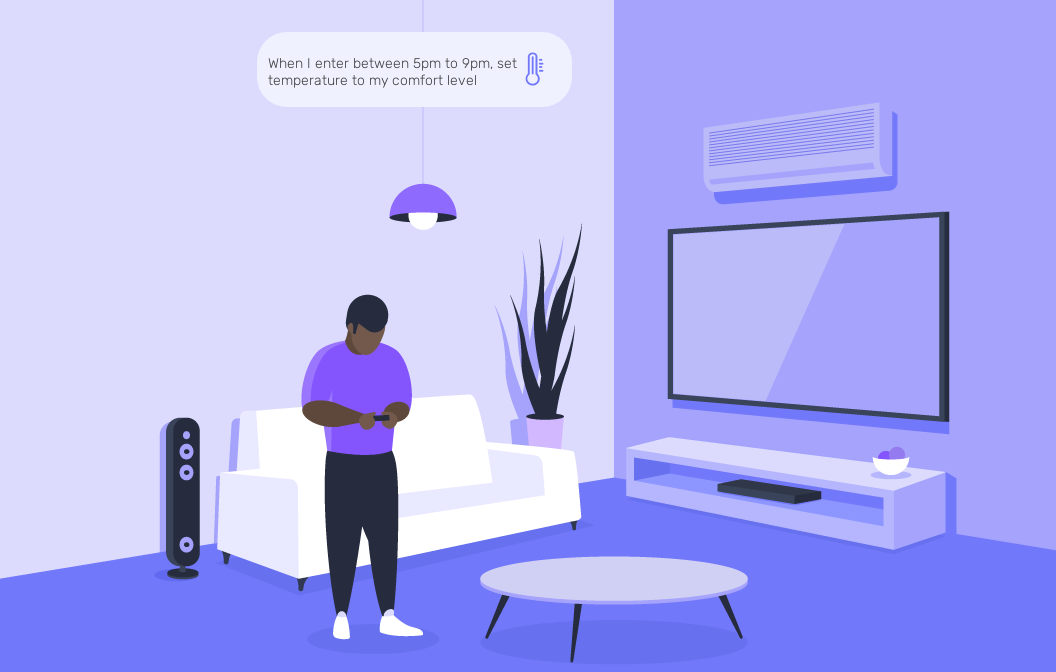
\includegraphics[width=\textwidth]{images/1.png}
\end{frame}

%%%%%%%%%%%%%%%%%%%%%%%%%%%%%%%%%%%%%%%%%%%%%%%%%%%%%%%%%%%%%%%%%%%%%%%%%%%%%%%%%%%%%%%%%%%%%%%%

\section{Interview Plan}

%%%%%%%%%%%%%%%%%%%%%%%%%%%%%%%%%%%%%%%%%%%%%%%%%%%%%%%%%%%%%%%%%%%%%%%%%%%%%%%%%%%%%%%%%%%%%%%%

\begin{frame}{Experts}
	\begin{itemize}
        \pause{}
		\item
		\pause{}
		\item
		\pause{}
		\item
	\end{itemize}	
\end{frame}

%%%%%%%%%%%%%%%%%%%%%%%%%%%%%%%%%%%%%%%%%%%%%%%%%%%%%%%%%%%%%%%%%%%%%%%%%%%%%%%%%%%%%%%%%%%%%%%%

\begin{frame}{Questions I.}
	\begin{itemize}
        \pause{}
		\item
		\pause{}
		\item
		\pause{}
		\item
		\pause{}
		\item
		\pause{}
		\item
	\end{itemize}	
\end{frame}

%%%%%%%%%%%%%%%%%%%%%%%%%%%%%%%%%%%%%%%%%%%%%%%%%%%%%%%%%%%%%%%%%%%%%%%%%%%%%%%%%%%%%%%%%%%%%%%%

\begin{frame}{Questions II.}
	\begin{itemize}
        \pause{}
		\item
		\pause{}
		\item
		\pause{}
		\item
		\pause{}
		\item
		\pause{}
		\item
	\end{itemize}	
\end{frame}

%%%%%%%%%%%%%%%%%%%%%%%%%%%%%%%%%%%%%%%%%%%%%%%%%%%%%%%%%%%%%%%%%%%%%%%%%%%%%%%%%%%%%%%%%%%%%%%%

\begin{frame}{Questions III.}
	\begin{itemize}
        \pause{}
		\item
		\pause{}
		\item
		\pause{}
		\item
		\pause{}
		\item
		\pause{}
		\item
	\end{itemize}	
\end{frame}

%%%%%%%%%%%%%%%%%%%%%%%%%%%%%%%%%%%%%%%%%%%%%%%%%%%%%%%%%%%%%%%%%%%%%%%%%%%%%%%%%%%%%%%%%%%%%%%%
	%{\footnotesize \printbibliography}
  

%%%%%%%%%%%%%%%%%%%%%%%%%%%%%%%%%%%%%%%%%%%%%%%%%%%%%%%%%%%%%%%%%%%%%%%%%%%%%%%%%%%%%%%%%%%%%%%%

\end{document}
